% Options for packages loaded elsewhere
\PassOptionsToPackage{unicode}{hyperref}
\PassOptionsToPackage{hyphens}{url}
%
\documentclass[
]{book}
\usepackage{amsmath,amssymb}
\usepackage{iftex}
\ifPDFTeX
  \usepackage[T1]{fontenc}
  \usepackage[utf8]{inputenc}
  \usepackage{textcomp} % provide euro and other symbols
\else % if luatex or xetex
  \usepackage{unicode-math} % this also loads fontspec
  \defaultfontfeatures{Scale=MatchLowercase}
  \defaultfontfeatures[\rmfamily]{Ligatures=TeX,Scale=1}
\fi
\usepackage{lmodern}
\ifPDFTeX\else
  % xetex/luatex font selection
\fi
% Use upquote if available, for straight quotes in verbatim environments
\IfFileExists{upquote.sty}{\usepackage{upquote}}{}
\IfFileExists{microtype.sty}{% use microtype if available
  \usepackage[]{microtype}
  \UseMicrotypeSet[protrusion]{basicmath} % disable protrusion for tt fonts
}{}
\makeatletter
\@ifundefined{KOMAClassName}{% if non-KOMA class
  \IfFileExists{parskip.sty}{%
    \usepackage{parskip}
  }{% else
    \setlength{\parindent}{0pt}
    \setlength{\parskip}{6pt plus 2pt minus 1pt}}
}{% if KOMA class
  \KOMAoptions{parskip=half}}
\makeatother
\usepackage{xcolor}
\usepackage{longtable,booktabs,array}
\usepackage{calc} % for calculating minipage widths
% Correct order of tables after \paragraph or \subparagraph
\usepackage{etoolbox}
\makeatletter
\patchcmd\longtable{\par}{\if@noskipsec\mbox{}\fi\par}{}{}
\makeatother
% Allow footnotes in longtable head/foot
\IfFileExists{footnotehyper.sty}{\usepackage{footnotehyper}}{\usepackage{footnote}}
\makesavenoteenv{longtable}
\usepackage{graphicx}
\makeatletter
\def\maxwidth{\ifdim\Gin@nat@width>\linewidth\linewidth\else\Gin@nat@width\fi}
\def\maxheight{\ifdim\Gin@nat@height>\textheight\textheight\else\Gin@nat@height\fi}
\makeatother
% Scale images if necessary, so that they will not overflow the page
% margins by default, and it is still possible to overwrite the defaults
% using explicit options in \includegraphics[width, height, ...]{}
\setkeys{Gin}{width=\maxwidth,height=\maxheight,keepaspectratio}
% Set default figure placement to htbp
\makeatletter
\def\fps@figure{htbp}
\makeatother
\setlength{\emergencystretch}{3em} % prevent overfull lines
\providecommand{\tightlist}{%
  \setlength{\itemsep}{0pt}\setlength{\parskip}{0pt}}
\setcounter{secnumdepth}{5}
\ifLuaTeX
  \usepackage{selnolig}  % disable illegal ligatures
\fi
\usepackage[]{natbib}
\bibliographystyle{apalike}
\IfFileExists{bookmark.sty}{\usepackage{bookmark}}{\usepackage{hyperref}}
\IfFileExists{xurl.sty}{\usepackage{xurl}}{} % add URL line breaks if available
\urlstyle{same}
\hypersetup{
  pdftitle={Template Study Note V2.0},
  pdfauthor={Author: Jung Xue},
  hidelinks,
  pdfcreator={LaTeX via pandoc}}

\title{Template Study Note V2.0}
\author{Author: Jung Xue}
\date{Last Updated: 2024-04-09}

\begin{document}
\maketitle

{
\setcounter{tocdepth}{1}
\tableofcontents
}
\hypertarget{ch1}{%
\chapter{Investments and securities markets}\label{ch1}}

•describe differences among asset classes and construction of stock market indexes, and calculate profit/loss on options/futures investments.
•describe how firms issue securities, and identify types of investors' orders
•compare mechanics and implications of buying on margin \& short selling
•cite pros/cons of investing with an investment company, and contrast open end mutual funds with other types of investment companies.
•define net asset value (NAV) and measure the rate of return on a mutual fund, and classify mutual funds according to investment style.
•demonstrate the impact of expenses and turnover on fund performance

\hypertarget{asset-classes-and-financial-instruments}{%
\section{Asset Classes and Financial Instruments}\label{asset-classes-and-financial-instruments}}

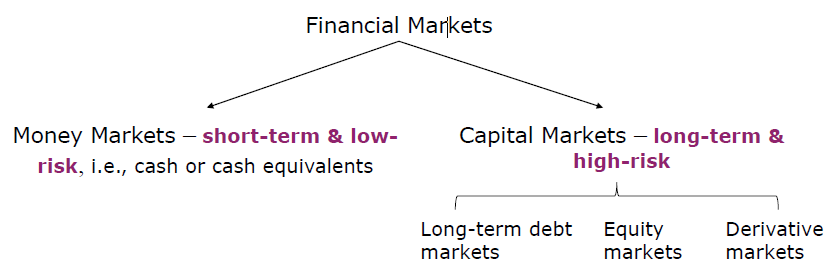
\includegraphics{Resources/Financialmarkets.png}
\#\#\# Money Markets

-- Treasury bills
-- Certificates of deposits (term deposits)
-- Commercial Paper CP (short term unsecured corporate notes)
-- Bankers Acceptances (a postdated check)
-- Eurodollars (U.S. dollar denominated deposits at foreign banks or foreign branches of U.S. banks)
-- Repurchase Agreements (Repos or RPs) and Reverse Repos.
-- Others, e.g., Brokers ' Calls interests charged by banks on loans made to brokerage firms), Federal Funds, The LIBOR Market, and Money Market Funds

\hypertarget{the-bond-market}{%
\subsection{The bond market}\label{the-bond-market}}

\begin{itemize}
\tightlist
\item
  Treasury Notes/Bonds (\$21 billion, \$21/\$51= 41\% of 2020 US Bond Market)
\item
  Mortgages and Mortgage Backed Securities (\$12.7 billion, 25\%
\item
  Corporate Bonds, including secured bonds, debentures (unsecured), callable/puttable/convertible bonds (\$10.6 billion, 21\%
\item
  Municipal Bonds (Issued by states/local, tax exempt) (\$3.95 billion, 7.8\%)
\item
  Federal Agency Debt, e.g., Fannie Mae, Freddie Mac ( 3.3\%)
\item
  International Bonds

  \begin{itemize}
  \tightlist
  \item
    Eurobonds: Eurodollar bonds bonds denominated in a currency other than the issuer's currency
  \item
    Yankee bond: US dollar denominated bond sold in the U.S. by a non U.S. issuer
  \end{itemize}
\item
  Inflation Protected Bonds (i.e., principal is adjusted per CPI)
\end{itemize}

\hypertarget{the-equity-market}{%
\subsection{The equity market}\label{the-equity-market}}

\begin{itemize}
\tightlist
\item
  Common stocks
\item
  Preferred stocks (behaving to bond)
\item
  Depository receipts, (shares in a foreign company)
\end{itemize}

\hypertarget{stock-and-bond-market-indexes}{%
\subsection{Stock and bond market indexes}\label{stock-and-bond-market-indexes}}

\begin{itemize}
\item
  Broad based index (S\&P 500 etc.)
\item
  Narrow based index (composed of only a few stocks, in a specific industry)
\item
  Why indexes?
\item
  Provide performance benchmarks
\item
  Base of derivatives
  -``Smart beta''
\end{itemize}

Construction Methodology:
- Price weighted (DJIA)
- Market value weighted (S\&P500, NASDAQ)
- Equal weighted (simple average of returns)

\hypertarget{derivative-markets}{%
\subsection{Derivative markets}\label{derivative-markets}}

\begin{itemize}
\tightlist
\item
  A security with a payoff that depends on the prices of other securities
\item
  Call/put options
\item
  Futures/Forwards
\item
  Swaps, futures options, etc.
\item
  Why we need them?
\item
  Speculative
\item
  Hedging
\item
  Arbitraging
\end{itemize}

\hypertarget{securities-markets-and-trading}{%
\section{Securities Markets and Trading}\label{securities-markets-and-trading}}

Originators
- Publicly traded companies initial public offering (IPO), and seasonal equity offerings (SEOs), - Privately held firms (private placement in which shares are sold directly to
a small group of institutional or wealthy investors)
- Shelf registrations (public firms can register securities and gradually sell them to the public )

How securities are traded (in secondary markets)
- Direct search (e.g.~painting)
- Brokered
- Dealer
- Auctions

\hypertarget{trading-mechanisms}{%
\section{Trading mechanisms}\label{trading-mechanisms}}

\hypertarget{over-the-counter-dealer-markets-otc-markets}{%
\section{Over the counter dealer markets (OTC Markets)}\label{over-the-counter-dealer-markets-otc-markets}}

Electronic communication networks ( ECNs)
\#\# Market Participants

\hypertarget{ch2}{%
\chapter{Enter Chapter title here}\label{ch2}}

\hypertarget{enter-subsection-1-here}{%
\section{Enter subsection 1 here}\label{enter-subsection-1-here}}

\hypertarget{enter-subsection-2-here}{%
\section{Enter subsection 2 here}\label{enter-subsection-2-here}}

\hypertarget{ch3}{%
\chapter{Enter Chapter title here}\label{ch3}}

\hypertarget{enter-subsection-1-here-1}{%
\section{Enter subsection 1 here}\label{enter-subsection-1-here-1}}

\hypertarget{enter-subsection-2-here-1}{%
\section{Enter subsection 2 here}\label{enter-subsection-2-here-1}}

\hypertarget{ch4}{%
\chapter{Enter Chapter title here}\label{ch4}}

\hypertarget{enter-subsection-1-here-2}{%
\section{Enter subsection 1 here}\label{enter-subsection-1-here-2}}

\hypertarget{enter-subsection-2-here-2}{%
\section{Enter subsection 2 here}\label{enter-subsection-2-here-2}}

\hypertarget{ch5}{%
\chapter{Enter Chapter title here}\label{ch5}}

\hypertarget{enter-subsection-1-here-3}{%
\section{Enter subsection 1 here}\label{enter-subsection-1-here-3}}

\hypertarget{enter-subsection-2-here-3}{%
\section{Enter subsection 2 here}\label{enter-subsection-2-here-3}}

\hypertarget{ch6}{%
\chapter{Enter Chapter title here}\label{ch6}}

\hypertarget{enter-subsection-1-here-4}{%
\section{Enter subsection 1 here}\label{enter-subsection-1-here-4}}

\hypertarget{enter-subsection-2-here-4}{%
\section{Enter subsection 2 here}\label{enter-subsection-2-here-4}}

\hypertarget{ch7}{%
\chapter{Enter Chapter title here}\label{ch7}}

\hypertarget{enter-subsection-1-here-5}{%
\section{Enter subsection 1 here}\label{enter-subsection-1-here-5}}

\hypertarget{enter-subsection-2-here-5}{%
\section{Enter subsection 2 here}\label{enter-subsection-2-here-5}}

\hypertarget{ch8}{%
\chapter{Enter Chapter title here}\label{ch8}}

\hypertarget{enter-subsection-1-here-6}{%
\section{Enter subsection 1 here}\label{enter-subsection-1-here-6}}

\hypertarget{enter-subsection-2-here-6}{%
\section{Enter subsection 2 here}\label{enter-subsection-2-here-6}}

\hypertarget{ch9}{%
\chapter{Enter Chapter title here}\label{ch9}}

\hypertarget{enter-subsection-1-here-7}{%
\section{Enter subsection 1 here}\label{enter-subsection-1-here-7}}

\hypertarget{enter-subsection-2-here-7}{%
\section{Enter subsection 2 here}\label{enter-subsection-2-here-7}}

\hypertarget{ch10}{%
\chapter{Enter Chapter title here}\label{ch10}}

\hypertarget{enter-subsection-1-here-8}{%
\section{Enter subsection 1 here}\label{enter-subsection-1-here-8}}

\hypertarget{enter-subsection-2-here-8}{%
\section{Enter subsection 2 here}\label{enter-subsection-2-here-8}}

\hypertarget{ch11}{%
\chapter{Enter Chapter title here}\label{ch11}}

\hypertarget{enter-subsection-1-here-9}{%
\section{Enter subsection 1 here}\label{enter-subsection-1-here-9}}

\hypertarget{enter-subsection-2-here-9}{%
\section{Enter subsection 2 here}\label{enter-subsection-2-here-9}}

\hypertarget{ch12}{%
\chapter{Enter Chapter title here}\label{ch12}}

\hypertarget{enter-subsection-1-here-10}{%
\section{Enter subsection 1 here}\label{enter-subsection-1-here-10}}

\hypertarget{enter-subsection-2-here-10}{%
\section{Enter subsection 2 here}\label{enter-subsection-2-here-10}}

\hypertarget{concluding-remarks}{%
\chapter*{Concluding Remarks}\label{concluding-remarks}}
\addcontentsline{toc}{chapter}{Concluding Remarks}

\hypertarget{three-points-learnt}{%
\section*{Three points learnt}\label{three-points-learnt}}
\addcontentsline{toc}{section}{Three points learnt}

Summarise three major point that you learnt from this course:

\begin{itemize}
\tightlist
\item
\item
\item
\end{itemize}

\hypertarget{three-questions-to-ask}{%
\section*{Three questions to ask}\label{three-questions-to-ask}}
\addcontentsline{toc}{section}{Three questions to ask}

Come up with three questions to ponder:

\begin{itemize}
\tightlist
\item
\item
\item
\end{itemize}

\hypertarget{remarks}{%
\section*{Remarks}\label{remarks}}
\addcontentsline{toc}{section}{Remarks}

\begin{itemize}
\tightlist
\item
\end{itemize}

\hypertarget{how-to-use-rbookdown}{%
\chapter*{How to use RBookDown}\label{how-to-use-rbookdown}}
\addcontentsline{toc}{chapter}{How to use RBookDown}

Firstly, you will have to read the \href{https://bookdown.org/yihui/bookdown/}{RBookDown Bible} by YiHui Xie

In essence, you write in a mixture of markdown (For basics), html (to extend on markdown) and latex language (mostly for equations) to create a simple Note.

You can customise your style and theme through your own CSS.

RMarkdown are mostly used to knit e-books(HTML), use TexStudio if you want a proper PDF, it is easier.

\textbf{Here are some useful tips to get started}

1: To add a chapter, just open a R file and save as \texttt{.RMD}. Use number 0 to 99 with a hyphen \texttt{-} to order the RMD files and maybe add a Chapter name so it is easier to select from \texttt{Files} window at bottom right of the R Studio.

2: Code chunks can generate graphical outputs, To insert pictures just use \texttt{include\_graphics} instead of \texttt{\textbackslash{}includegraphics\{\}} or \texttt{!{[}{]}()}. Width can be customised.

\begin{verbatim}
knitr::include_graphics(rep('images/knit-logo.png', 3))
\end{verbatim}

3: Use 1 grave accent ` to include the in line code, use 3 grave accent to include a chunk of code.

  \bibliography{references.bib}

\end{document}
